%!TeX program=pdflatex
%!TeX encoding=utf8
%!TeX spellcheck = en_GB
%!TeX root = ../../messageVortex.tex

\part{Results}
To verify the hypothesis made in this paper, and to analyse properties of the protocol in a real world scenario a library was implemented in Java which was capable of handling all message packets and the routing stack as a whole. The following paragraphs describe the protocol developed in general as a generic approach. Appendix \ref{app:asnone} gives the full ASN.1 representation of the protocol. 

It is important to notice that ASN.1 has no mean to express encrypted structures. Due to this fact we defined all encrypted fields as \verb|OCTET STRING|. 

The protocol is defined int the ASN.1 to support onionized information in an unencrypted form. This is meant for debugging purposes only. At no point should this possibility be used in a production environment.

The protocol described in the next chapter is independent from routing. We built a blending layer for SMTP. Layers for other protocols such as XMMP may be built similarly. The protocol may be extended by adding blending layers and their addressing schemes.

\chapter{Vortex Prerequisites}
\section{Hardware}

\fxfatal{add content here}

\section{Addresses}
A Vortex address is built as follows: $vortexAddress=<transport>:<address>!<publicKey>$

To allow storage of Vortex addresses sin standard messaging programs such as Outlook or Thunderbird. We define an alternate representation $encodedVortexAddress=base64(vortexAddress)@localhost$. 

The suffix ``@localhost'' makes sure that a message intended for Vortex is not routed by any non-participating server.

The main downside of vortex addresses are that they are no longer readable by a human. The main reason for this is the public key which is required. We may abstract this further by allowing clear text requests on the main email address for the public key. Such requests must then be answered by the vortex account with the valid Vortex address.

\section{Client}
We did not create a Vortex client for sending messages. Instead we used a standard Thunderbird email client pointing to a local SMTP and IMAP Server provided by Vortex. On the SMTP side Vortex does encapsulate where possible mails into a Vortex message and builds automated route to the recipient. The SMTP part of vortex may be used to encapsulate automatically all messages with a known Vortex identity into a vortex message. On the IMAP side it merges a local Vortex message store with the standard Email repository building a combined view.

Using Vortex like this offers us the advantages of a known client with the anonymity Vortex offers.

This has certain downsides. At the moment the vortex client has only a local store this makes it impossible to handle multiple simulatneously connected clients to use Vortex. This is however just a lack of the current implementation and not of the protocol itself as we may safely use an IMAP storage for storing vortex mails centrally.

\subsection{Vortex Accounts}
By definition any transport layer address may represent a Vortex identity. This fact may make people believe that their current email or jabber address is suitable as Vortex address. This is technically perfectly true, but should not be done for the following reasons:

\begin{itemize}
	\item If an address is identified as a vortex address it may be blocked (directly or indirectly) by an adverser.
	\item If a vortex node is malfunctioning non-vortex messages should remain unaffected. This is more likely to happen if non-Vortex messages are kept in a separate account.
	\item If a user wants no longer to maintain its Vortex address (hopefully there will be a better technology in future) he just may give up his Vortex accounts. If he would have been using his normal messaging account for Vortex he would receive mixing messages which he has to filter in future.
\end{itemize}

\subsection{Vortex Node Types}

\subsubsection{Public Vortex Node}
Public nodes are nodeswhich advertise themself as mixes. Just as all nodes they may be an endpoint or a mix. Typically they accept all requests exactly as outlined in \ref{tab:protoReplyCrit}. As an immediate result of the publicly available information about such a node the owner may be target of our adverser. Pressure may be oposed to close down such a node. However since we do not need a specific account we may safely close down one transport account and open up a different one (on the same or a different infrastructure).

\subsubsection{Stealth Vortex Node}
This node does not answer any clear text requests. As an immediate result the node is only usable by other nodes knowing the public key of this node. The node is therefore on a known secret base only reachable.

\subsubsection{Hidden Vortex Node}
A hidden node is a special form to a stealth node it has a set of preset identities. Only these entities are processed. This behaveour has certain drawbacks. An identity may not be changed. As an immediate result traffic may become a pseudonymity. To counter this effect at least partially we may use the same local identity for multiple senders. As an immediate result the sender is only one of all senders knowing the private key of an identity.

\chapter{MessageVortex - Transport Independent Messaging anonymous to \nth{3} Parties}
This approach is different from all approaches discussed previously. Unlike them we put complete distrust into the infrastructure being used. Furthermore we do not rely on a custom server infrastructure in the internet. Instead we take advantage of the availability of internet connected devices such as internet connected mobile phones, tablets, or even commonly available SoC such as RaspberryPi or similar. It is still very hard to maintain a server in the internet and considering the vastly growing amount of automated attack carried out against internet connected servers it is not advisable or realistic to assume that a future user of this system owns either a server or connects to a service which is offering explicitly anonymizing services. These infrastructures would be suspectible to monitoring or even banning. Instead we take a different approach.

We use common messaging protocols as transport layers and connect to them using the respective client protocols. The actual mixes are operated by the users on their ``always connected'' devices. It goes without saying that such a system is far less reliable than a traditionally run server as this hardware is typically cheap and normally connected to the internet using a bandwidth shared media.

The basic idea is that a client generates all traffic (including decoy or dummy traffic) by itself. It defines the routes a message takes through the mixes and decides which targets are receiving dummy traffic at the same time. In such a system even when possessing all the nodes routing the traffic (without the endpoints) an anonymity set of $k$ (whereas the size of $k$ is defined by the sender) is guaranteed.

As decoy traffic is generated with the same operations as the true content is split it is impossible for an adverser running a node to determine whether he is generating noise or actually processing the true message.

\fxfatal{add a lot more text here}
\begin{figure}[h]
	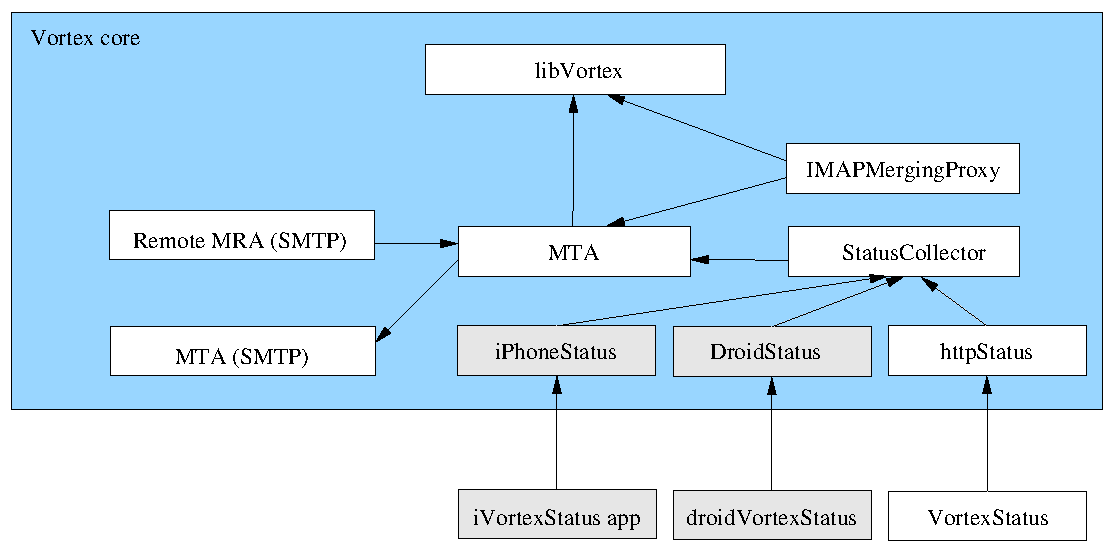
\includegraphics[width=\columnwidth]{inc/VortexModules.pdf}
	\caption{Overview of the Vortex modules}
	\label{fig:vortexModules}
	\fxfatal{replace image with up to date representation; show implemented and not implemented parts; Maybe make it two column wide}
\end{figure}

\section{Protocol Implementation\label{protoImpl}}
\fxfatal{add content here}

\section{Block Structure}
\lstinputlisting[language=ASN1, caption={Header Block}, backgroundcolor=\color{gray!10},linerange={29-71},firstnumber=29]{../app/asn.1/messageBlocks.asn} 

\subsection{Header Block}
\fxfatal{add content here}

\subsection{Routing Blocks}
\fxfatal{add content here}

\subsection{Payload Blocks}
\fxfatal{add content here}

\section{Message Building}
\fxfatal{take care of percentage and floating point precision}


\section{Accounting}
In table \ref{tab:protoReplyCrit} we show under what circumstances a reply to a header request should be sent. The capitalised words MAY, MUST, SHOULD and SHOULD NOT are used as defined in RFC2119\cite{RFC2119}.
\begin{table*}[h]
	\centering\scriptsize
	\begin{tabular}{|l|l|l|l|l|}\hline
		\diaghead{\theadfont Request Criteria}{Request}{Criteria} & \thead{unknown identity; cleartext} & \thead{unknown identity; encrypted} & \thead{expired identity; encrypted} & \thead{known identity; encrypted}\\\hline
		newIdentity	 	& SHOULD NOT 	& SHOULD NOT& Invalid (Error) 	& Invalid (Error)\\              
		queryPeer       & MUST NOT      & MUST NOT  & MAY               & MAY\\        
		queryCapability	& SHOULD 		& MUST 		& MUST				& MUST \\
		messageQuota	& MUST NOT 		& MUST NOT	& MAY				& MUST \\              
		transferQuota	& MUST NOT		& MUST NOT	& MAY				& MUST \\\hline             
	\end{tabular}	
	\caption{Requests and the applicable criteria for replies}
	\label{tab:protoReplyCrit}
\end{table*}

\fxfatal{add content here}

\section{Blending layer}
\fxfatal{add content here}

\section{Message Flows}
\fxfatal{add content here}

\section{Considerations for Building Messages}
In a worst case scenario we assume that an adverser is controlling most of the network utilized for anonymisation. While this is not necessarily a problem (as pointed out earlier) it allows an adverser to track a message while agents are being used under his control. So for simplicity and as a worst case assumption we always assume that an adverser has perfect knowledge of an associated message flow. This is however a worst case scenario. One missing agent disconnects the whole chain and as messages are not traceable in size.

\fxfatal{add selffailing operations as checkpoint}

\subsection{Ephemeral identities}
\fxfatal{expiring ephemeral identities should not only be replaced after their expiration but anytime during the livetime}

\subsection{Timing of messages}
\fxfatal{add content here}

\subsection{Diagnostics}
\fxfatal{add content here}

\subsubsection{Implicit Diagnostic}
\fxfatal{Add comments about messages splitting and returning to sender}

\subsubsection{Automatic Explicit Diagnostic}
\fxfatal{Add comments about error and diagnosis messages officially spliting of messages}

\subsubsection{On-Demand Explicit Diagnostic}
\fxfatal{Add comments about normal, error, and diagnosis messages being picked up by a routing block}

\section{Verification of requirements}
In the previous sections we identified the following list of requirements:
\slistofrequirements
In the following subsections we will iterate through all requirements and verify to what degree we achieved the goal.

\fxfatal{list all requirements}

\paragraph{\ref{req:zeroTrust}:} 
We have not put any trust intu an external infrastructure. While we do assume that all routing nodes act as defined. A misbehaving node may be identified and eliminated without putting any trust on other nodes. Analysis have shown no means for a misbehaving node which might be intentional or unintentional endangering anonymity at any time. We do not rely on any third party technology or infrastructure for our anonymity. 

This requirement is therefore fulfilled.

\paragraph{\ref{req:P2P}:} 
No node has additional privileges or offers additional services. All are equal and share the same privileges.

This requirement is therefore fulfilled.

\paragraph{\ref{req:untagable}:} 
Messages may not be tagged. All content is either strictly onionised or defined and linked with unknown hooks. Tampering with a message will cause the message delivery to fail at the next node.

This requirement is therefore fulfilled.
 
\paragraph{\ref{req:unbugable}:} 
There are always means to bug a message. As we put trust in sender and recipient and we know already that a intermediate mixing node is not able to modify the message the protocol is hard to bug. There may be a possibility to bug a message with a routing log entry over DNS. If a recipient is not resolving names or trusts in the content of such a message he is safe.

This requirement is therefore fulfilled.
\paragraph{\ref{req:replay}:} 

\fxfatal{add content}
\paragraph{\ref{req:accounting}:} 

\fxfatal{add content}
\paragraph{\ref{req:anon}:} This point is the hardest to proof. We certaindly achieved a high degree of anonymity. No node can tell by observing traffic if a node is a final recipient or just a mix. There are however some weaknesses in the protocol. As the implementation is currently connecting simultaneously to the tru named and the Vortex account the user might be identified by that fact. Using a anonymisation proxy could solve the problem but it would violate the Zero trust principle.

\paragraph{\ref{req:boot}:} 

\fxfatal{add content}
\paragraph{\ref{req:cryptVar}:} 

\fxfatal{add content}

\paragraph{\ref{req:easy}:}

\fxfatal{add content}

\section{Considerations for Routing Messages}
\subsection{Time of sending}
Messages should always be sent timewise nearby other messages. This means that the best moment for sending a message in a ready queue is at a time when sending of other messages is due. However no optimisation should be done to send as many messages as possible at the same time. this would lead to a forseeable behaviour of the routing layer and thus to misusable behaviour.

\section{Real World Considerations}
This approach is heavily dependent of the transport protocol and builds on top a new obfuscating/routing layer. For this system to become a real peer-to-peer approach some additional quirks are required. A message-Vortex-Account needs always an active routing handler. This routing handler may be introduced by new server capabilities or by having a device handling the routing from the client side. For this reason we built a RaspberryPi appliance capable of connecting to one (or more) accounts fetching incomming mails, analysing them and reroute them if necessary. Although the system is designed to be run on a RaspberryPi the software might be installed to any Java capable client. The RaspberryPi is just one affordable lightweight device which offers all required capabilities.

\subsection{No Routing Log}
There was up until very late a routing log functionality in the protocol. This functionality did however have the disadvantage that it allowed bugging and could possibly  disclose intermediate mixes to a recipient which did not comply with the policy the mixes might have chosen. Therefore this feature was dropped and replaced with the fetch block behaviour.

\subsection{Message Content}
\fxfatal{add content here}

\chapter{Security Analysis}
In the following sections we emphasize on attacks targeting either sender recipient tuples or on identification of participants. 

Based on the protocol we may safely assume the following key ponts:
\begin{itemize}
	\item An adverser knows and controls a significant number of nodes (for our analysis we assume less than 80\%).
	\item An adverser may observe the traffic at any point without getting any information about the message content
	\item An adverser is not capable of matching multiple messages on different nodes to one message.
\end{itemize}

We always assume an adverser to have more knowledge than we think he may extract from the messages.
\begin{itemize}
	\item We assume that an adverser knows all messages of a transaction running over his nodes and matches them correctly to the same message.
	\item 
\end{itemize}

We assume that the adverser is targeting the following informations:
\begin{itemize}
	\item Sender identity
	\item Recipient identity
	\item Message content
	\item Message size
\end{itemize}

\subsection{Attack on Users Identity}
\fxfatal{add content here}

\subsubsection{Frequency and Bandwidth Analysis}
\fxfatal{add content here}

\subsection{Attack on Message content}
\fxfatal{add content here}

\subsubsection{Attacking Routing Blocks}
\fxfatal{add content here}

\subsection{Attack on Message size}

\fxfatal{add content here}

\chapter{Additional Considerations}
\section{Man in the Middle Attacks to Conversations}

\fxfatal{add content here}

\section{Identification of participating account}

\fxfatal{add content here}

\subsection{Identification by content}
It is possible to identify a message by content. Assuming that an adverser knows the applied blending methode he may identify an ASN.1 structure of 

\fxfatal{add content here}

\subsection{Identification by Query}

\fxfatal{add content here}

\subsection{Identification by Traffic Type}

\fxfatal{add content here}

\subsection{Identification by Bandwidth}

\fxfatal{add content here}

\subsection{Identification by Behavioural analysis}

\fxfatal{add content here}

\section{Storage of Messages and queues}
The storage of messages sent though MessageVortex should be handled with great care. It seems on the first sight a good idea to merge all messages in a globally available storage such as the mail account of the receiving entity. However -- In doing so we would discover the message content to the providing party of a mail account. Since we handled the message with great care and tremendous costs up until this point it would be careless doing so. 

Storing them in a localized and receiving entity controlled storage is definitely a good idea but leaves security considerations like a backup possibly to an end user. This might be better but in effect a questionable decision. There is however a third option. By leaving the message unhandled on the last entity of the MessageVortex chain we may safely backup the data without disclosing the message content. Merging the content then dynamically through a specialized proxy would allow the user tu have a unified view on his without compromising the security.

\fxfatal{implemented in prototype?}

\section{Economy of transfer}

\fxfatal{Write something about wasting bandwidth}